\documentclass[10pt]{article}


\usepackage {
  amsmath,
  amssymb,
  amsthm,
  array,
  graphicx,
  multicol,
  longdivision
}

\usepackage[colorlinks=true]{hyperref}
\usepackage[dvipsnames]{xcolor}
\usepackage[english]{babel}
\usepackage[margin=1in]{geometry}
\usepackage[utf8]{inputenc}
\usepackage{color}
\usepackage{circuitikz}

\hypersetup {
  citecolor = ForestGreen,
  filecolor = Plum,
  linkcolor = NavyBlue,
  urlcolor = RubineRed
}

\newcommand{\C}{\mathbb{C}}
\newcommand{\F}{\mathbb{F}}
\newcommand{\Q}{\mathbb{Q}}
\newcommand{\Z}{\mathbb{Z}}
\newcommand{\R}{\mathbb{R}}
\newcommand{\N}{\mathbb{N}}
\newcommand{\CO}{\mathcal{O}}
\newcommand{\CC}{\mathcal{C}}
\newcommand{\CU}{\mathcal{U}}
\newcommand{\spacing}{\vspace*{1\baselineskip}}


\title{COMP
251:
Algorithms
and
Data
Structures
-
Proofs
Assignment}
\author{Student ID: 261102963}\\
\date{\today}


\begin{document}
  \maketitle


  \subsection*{Complexity Proof}


  Claim: Inserting a node $x$ into a red-black tree takes $O(log n)$ time.

  \subsubsection*{Presentation}


  \begin{proof}
    To prove that inserting a node $x$ into a red-black tree takes $O(log n)$ time,
    we need to show that the number of operations performed during the insertion
    operation is proportional to the height of the tree, which is $O(logn)$ as shown
    in the correctness proof.

    \spacing
    \noindent
    The insertion operation in a red-black tree can be divided into three main steps:

    \begin{enumerate}
      \item \textbf{Binary search tree insertion}: This step involves finding the
        correct position for the new node $x$ in the tree based on its key value,
        and inserting it as a regular binary search tree node.

      \item \textbf{Coloring the new node red}: The new node is colored red to preserve
        the red-black tree properties.

      \item \textbf{Fixing the red-black tree properties}: If the insertion of the
        new node causes a violation of the red-black tree properties, then one
        or more rotations and/or color flips are performed to restore the
        properties.
    \end{enumerate}

    \noindent
    Since step 1 involves a standard binary search tree insertion, the number of
    comparisons performed during this step is proportional to the height of the tree,
    i.e., $O(h)$. Therefore, the worst-case time complexity of step 1 is $O(h)$,
    which is $O(logn)$ in the average case for a balanced tree.

    \spacing
    \noindent
    Step 2 involves a constant number of operations, namely setting the color of
    the new node to red. Therefore, the time complexity of this step is $O(1)$.

    \spacing
    \noindent
    Step 3 involves fixing any violations of the red-black tree properties that
    may have occurred due to the insertion of the new node. The number of operations
    required to fix these violations is proportional to the height of the subtree
    affected by the violation. Since the subtree height is at most $h+1$, the worst-case
    time complexity of step 3 is $O(h+1)$, which is $O(log n)$ in the average
    case for a balanced tree.

    \spacing
    \noindent
    Therefore, the total worst-case time complexity of inserting a node into a red-black
    tree is $O(log n)$. This is because step 1 takes $O(log n)$, step 2 takes $O(
    1)$, and step 3 takes $O(log n)$. Therefore, the total number of operations
    is proportional to the height of the tree, which is $O(log n)$.
  \end{proof}

  \noindent
  Source: Slides

  \subsubsection*{Summary}


  The proof above shows that inserting a node $x$ into a red-black tree takes $O(
  logn)$ time. The insertion involves three steps: binary search tree insertion,
  coloring the new node red, and fixing any violations of the red-black tree properties.
  The time complexity of step 1 is $O(h)$, which is $O(logn)$ in the average case
  for a balanced tree (as shown in the correctness proof). Step 2 takes $O(1)$
  and step 3 takes $O(h+1)$, which is also $O(logn)$ in the average case.
  Therefore, the total worst-case time complexity of inserting a node into a red-black
  tree is $O(logn)$.

  \subsubsection*{Algorithm}


  Below you will find an algorithm that implements insertion for a red-black tree.
  The insertion algorithm includes the main three computational steps used in
  the proof, namely: BST insertion, coloring the new node red and fixing the red-black
  tree properties after the insertion was made. Many comments are made
  throughout the code to make things easier to understand. The full code includes
  a class $Node$ which defines a red-black tree node, $Tree$ which implements a
  small subset of red-black tree functionality and a $main$ method for testing
  out the insertion.

  \begin{verbatim}
    /*
     * Definition for a red-black tree node.
     */
    public class Node {
      int data;
      Node left, right, parent;
      boolean color;

      public Node(int data) {
        this.data = data;
      }

      public Node(int data, boolean color) {
        this.data = data;
        this.color = color;
      }
    }

    /*
     * A red-black tree with an insert operation.
     */
    public class Tree {
      Node root;

      static final boolean RED = false, BLACK = true;

      /*
       * Default constructor.
       */
      public Tree() {}

      /*
       * Constructor with root.
       *
       * @param root The root of the tree.
       */
      public Tree(Node root) {
        this.root = root;
      }

      /*
       * Insert a node into the red-black tree.
       *
       * => Simulates a normal BST insertion but finishes
       * with a fixUp subroutine for violated RB-tree properties.
       *
       * @param key The data the new node should have.
       */
      public void insert(int key) {
        Node node = root, par = null;

        // Depending on the key, we traverse left or right
        // => Same as in BST insertion.
        while (node != null) {
          par = node;
          if (key < node.data) node = node.left;
          else if (key > node.data) node = node.right;
          // Don't insert duplicate nodes
          else throw new IllegalArgumentException("Tree already contains a node with key " + key + ".");
        }

        // Color the new node red
        Node curr = new Node(key, RED);

        // Insert the node based on the key
        if (par == null) root = curr;
        else if (key < par.data) par.left = curr;
        else par.right = curr;

        // Set the parent of the newly inserted node
        curr.parent = par;

        // Fix the red-black tree properties
        fixUp(curr);
      }

      @Override
      public String toString() {
        StringBuilder builder = new StringBuilder();
        toStringHelper(root, builder);
        return builder.toString();
      }

      /*
       * Fix red-black tree properties after an insertion.
       *
       * @param node The node to initiate the fix from.
       */
      private void fixUp(Node node) {
        Node par = node.parent;

        // Case 1: If the parent is null, we've reached the root, which is the end of the recursion.
        // also, if the parent is black, there's nothing to do since the red-black properties are
        // preserved.
        if (par == null || par.color == BLACK) return;

        // From this point on, the parent is red.
        Node grandparent = par.parent;

        //// Case 2: If the grandparent is null, that means the parent is the root.
        // If we enforce black roots (rule 2), the grandparent will never be null.
        // => Just need to recolor the parent node
        //     R        B
        //      \   ->   \
        //       R        R
        if (grandparent == null) {
          // As this method is only called on red nodes, all we have to do is recolor the root black.
          par.color = BLACK;
          return;
        }

        // Grab the uncle of the parent node
        Node uncle = getUncle(par);

        // Case 3: If the uncle is red, recolor the parent, grandparent, and uncle.
        if (uncle != null && uncle.color == RED) {
          par.color = BLACK;
          grandparent.color = RED;
          uncle.color = BLACK;
          // Recursively fix the grandparent node
          fixUp(grandparent);
          // Parent is the left child of the grandparent.
        } else if (par == grandparent.left) {
          // Case 4a: If the uncle is black and the node is the right child of its parent (forming a
          // left-right zigzag pattern).
          if (node == par.right) {
            rotateLeft(par);
            // Update the parent pointer to the new root node of the rotated subtree.
            par = node;
          }
          // Case 5a: If the uncle is black and the node is the left child of its parent (forming a
          // left-left straight pattern).
          rotateRight(grandparent);
          // Recolor the original parent (now the root of the subtree) and grandparent.
          par.color = BLACK;
          grandparent.color = RED;

          // Parent is the right child of the grandparent.
        } else {
          // Case 4b: If the uncle is black and the node is the left child of its parent (forming a
          // right-left zigzag pattern).
          if (node == par.left) {
            rotateRight(par);
            // Update the parent pointer to the new root node of the rotated subtree.
            par = node;
          }
          // Case 5b: If the uncle is black and the node is the right child of its parent (forming a
          // right-right straight pattern).
          rotateLeft(grandparent);
          // Recolor the original parent (now the root of the subtree) and grandparent.
          par.color = BLACK;
          grandparent.color = RED;
        }
      }

      /*
       * Get the uncle node of a given input node.
       *
       * @param parent The node to grab the uncle from.
       * @return The uncle node.
       */
      private Node getUncle(Node parent) {
        Node grandparent = parent.parent;
        if (grandparent.left == parent) return grandparent.right;
        if (grandparent.right == parent) return grandparent.left;
        throw new IllegalStateException("Parent is not a child of its grandparent.");
      }

      /*
       * Perform a right tree rotation.
       *
       * @param node The node to rotate from.
       */
      private void rotateRight(Node node) {
        Node par = node.parent, left = node.left;
        node.left = left.right;
        if (left.right != null) left.right.parent = node;
        left.right = node;
        node.parent = left;
        replace(par, node, left);
      }

      /*
       * Perform a left tree rotation.
       *
       * @param node The node to rotate from.
       */
      private void rotateLeft(Node node) {
        Node par = node.parent, right = node.right;
        node.right = right.left;
        if (right.left != null) right.left.parent = node;
        right.left = node;
        node.parent = right;
        replace(par, node, right);
      }

      /*
       * Replace the child of the parent node.
       *
       * @param par The parent node.
       * @param oldChild The old child of the parent.
       * @param newChild The new child to replace the old child with.
       */
      private void replace(Node par, Node oldChild, Node newChild) {
        if (par == null) root = newChild;
        else if (par.left == oldChild) par.left = newChild;
        else if (par.right == oldChild) par.right = newChild;
        else throw new IllegalStateException("Node is not a child of its parent.");
        if (newChild != null) newChild.parent = par;
      }

      /*
       * A recursive helper method for building the toString
       * string builder.
       *
       * @param node The node to start from.
       * @param builder The string builder to append to.
       */
      private void toStringHelper(Node node, StringBuilder builder) {
        builder.append(node.data);

        if (node.left != null) {
          builder.append(" L{");
          toStringHelper(node.left, builder);
          builder.append("}");
        }

        if (node.right != null) {
          builder.append(" R{");
          toStringHelper(node.right, builder);
          builder.append("}");
        }
      }
    }

    /*
     * A small main program for testing out the insertion functionality.
     */
    public static void main(String[] args) {
      Tree tree = new Tree();

      for (int i = 0; i < 10; ++i) tree.insert(i);

      System.out.println(tree.toString());
    }
  \end{verbatim}

  \noindent
  n.b. Code adapted and repurposed from the following reference: \url{https://www.happycoders.eu/algorithms/red-black-tree-java/}

  \subsubsection*{Code explanation}


  Below is the time graph for red-black tree insertion. Setting aside outliers and
  system differences (ran this on an M2 Pro Macbook 32GB RAM), it generally
  agrees with the assigned $O(logn)$ time complexity.

  \newpage
  \vfill


  \begin{figure}[ht]
    \centering
    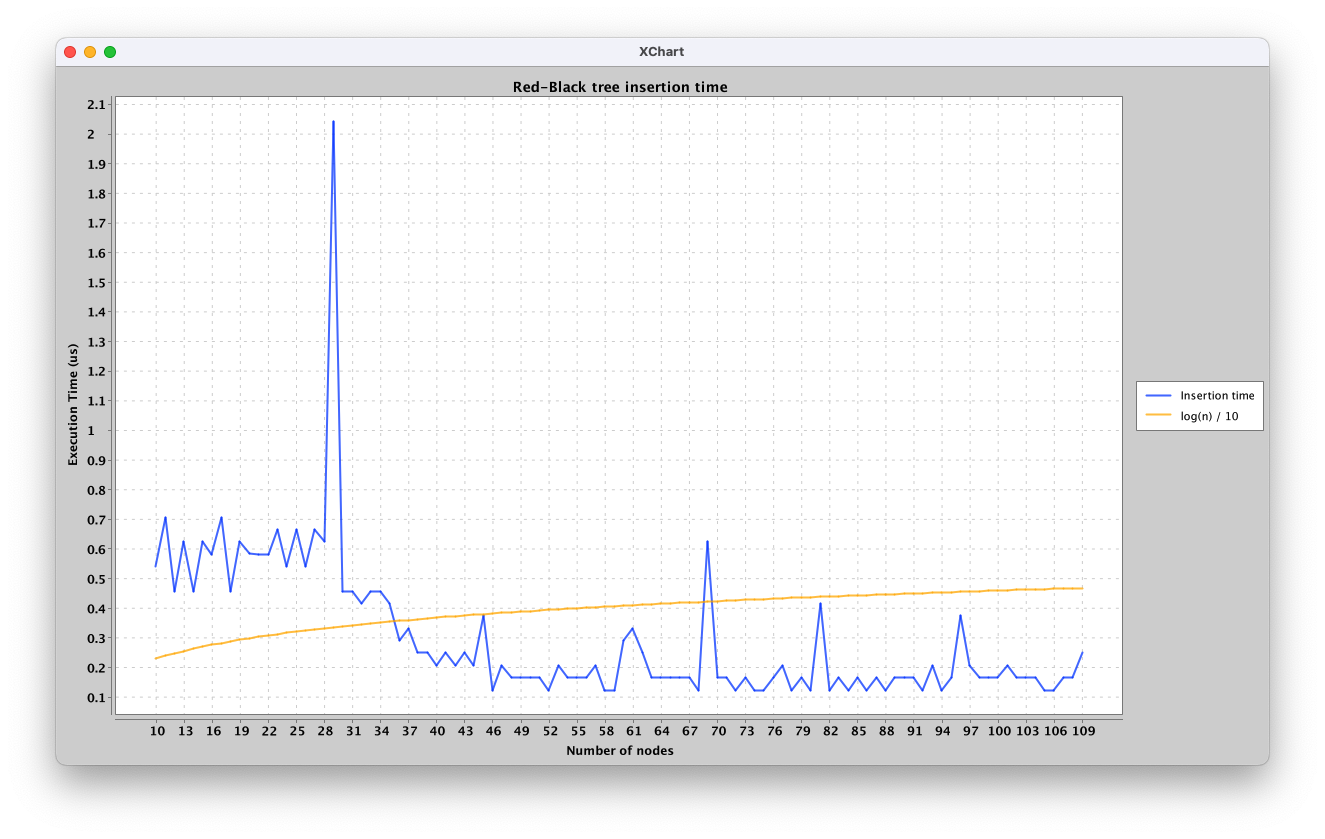
\includegraphics[width=1\textwidth]{complexity.png}
    \caption{Red-black tree insertion time graph}
    \label{fig:example}
  \end{figure}

  The above plot was generated with the following code (as provided in the java
  source files):

  \begin{verbatim}
    /*
     * Run insertion on a tree with a given number of nodes.
     *
     * @param n The number of nodes the tree should have.
     * @return The amount of time an insertion took.
     */
    static double runInsertion(int n) {
      Tree tree = new Tree();

      for (int i = 0; i < n; ++i) tree.insert(i);

      double start = System.nanoTime();
      tree.insert(n);
      double end = System.nanoTime();

      return (end - start) / 1000;
    }

    /*
     * Plot the insertion time chart.
     */
    static void plotChart() {
      int samples = 100;

      double[] x = new double[samples], y = new double[samples];

      int n = 10;

      for (int i = 0; i < samples; ++i) {
        System.out.println("Current iteration: " + i);
        y[i] = runInsertion(n);
        x[i] = n;
        n += 1;
      }

      XYChart chart =
          QuickChart.getChart(
              "Red-Black tree insertion time",
              "Number of nodes",
              "Execution Time (us)",
              "Insertion time",
              x,
              y);

      double[] y2 = new double[samples];

      for (int i = 0; i < samples; ++i) y2[i] = Math.log(x[i]) / 10;

      chart.addSeries("log(n) / 10", x, y2).setMarker(SeriesMarkers.NONE);

      new SwingWrapper<>(chart).displayChart();
    }
  \end{verbatim}

  \subsubsection*{Real world example}


  Red-black trees are a type of binary search tree that automatically balances
  itself. This makes them really useful in many computer science applications,
  including Database Management Systems (DBMS). When working with databases, it's
  important to have a good way to organize and search for information, which is where
  red-black trees come in.

  \spacing
  \noindent
  One way red-black trees are used in DBMS is through something called a B+ tree.
  This is a special kind of tree that works really well with computer storage and
  is better for searching through lots of data. In B+ trees, each node has a
  bunch of keys and pointers to other nodes, all sorted by the keys.

  \spacing
  \noindent
  When adding new data to the tree, you need to find the right place for it. You
  start at the top of the tree and follow the pointers based on how the new data
  compares to the keys in each node. Once you find the right spot in a leaf node,
  you add the new data there. If the node is already full, you need to split it up
  and make a new node, then move the middle key up to the parent node so
  everything stays organized.

  \spacing
  \noindent
  The cool thing about red-black trees (and B+ trees) is that they make sure the
  tree stays balanced, which means it takes less time to do things like search
  or add new data. Specifically, adding a new node to a red-black tree takes O(log
  n) time, where n is the number of entries in the tree. This is super important
  for large databases because it keeps operations running quickly.

  \spacing
  \noindent
  So, red-black trees are really helpful for organizing data in DBMS because
  they keep things balanced and make it easy to search, add, or delete data. They're
  the foundation for B+ trees, which are used a lot in DBMS to manage large databases
  efficiently.

  \spacing
  \noindent
  References:

  \begin{enumerate}
    \item Cormen, T. H., Leiserson, C. E., Rivest, R. L., & Stein, C. (2009).
      Introduction to Algorithms (3rd ed.). MIT Press.

    \item Ramakrishnan, R., & Gehrke, J. (2003). Database Management Systems (3rd
      ed.). McGraw-Hill.

    \item Bayer, R., & McCreight, E. M. (1972). Organization and Maintenance of
      Large Ordered Indices. Acta Informatica, 1(3), 173-189.
  \end{enumerate}

  \subsection*{Correctness Proof}


  Claim: A red-black tree with $n$ internal nodes has
  height at most $2log(n + 1)$.

  \subsubsection*{Presentation}


  \begin{proof}
    We start by showing that the subtree rooted at any node $x$ contains at least
    $2^{bh(x)}- 1$ internal nodes. We prove this claim by induction on the
    height of x. If the height of $x$ is 0, then x must be a leaf (T.nil), and the
    subtree rooted at $x$ indeed contains at least $2^{bh(x)}- 1$ = $2^{0}- 1$ =
    0 internal nodes. For the inductive step, consider a node $x$ that has positive
    height and is an internal node with two children. Each child has a black-height
    of either $bh(x)$ or $bhx - 1$, depending on whether its color is red or black,
    respectively. Since the height of a child of $x$ is less than the height of $x$
    itself, we can apply the inductive hypothesis to conclude that each child
    has at least $2^{bh(x) - 1}- 1$ internal nodes. Thus, the subtree rooted at
    $x$ contains at least ($2^{bh(x) - 1}- 1$) + ($2^{bh(x) - 1}- 1$) + 1 =
    $2^{bh(x)}- 1$ internal nodes, which proves the claim.
  \end{proof}

  \noindent
  Source: CLRS

  \subsubsection*{Summary}


  The proof shows that the height of a red-black tree with n internal nodes is
  at most 2 times the logarithm of $n+1$. The proof uses an idea called "black-height"
  which measures the number of black nodes on any path from the root to a leaf node.
  The proof shows that for any node $x$ in the tree, the subtree rooted at $x$ has
  at least twice the black-height of $x$, minus 1 internal nodes. This is proven
  by first showing that the claim is true for a node $x$ with height 0 (i.e., a
  leaf node), and then using induction to show that the claim is true for any
  node $x$ with positive height and two children. By adding up the minimum number
  of internal nodes in each child subtree, plus one for the current node, the proof
  shows that the subtree rooted at $x$ has at least twice the black-height of $x$,
  minus 1 internal nodes. This proves the original claim for the entire tree.

  \subsubsection*{Algorithm}


  Below is an algorithm for computing the height of a red-black tree (same as
  computing the height for a BST), note that I use the same code as above and
  these methods are present in the provided $Tree$ class.

  \begin{verbatim}
    ...

    /*
     * Compute the height of this red-black tree.
     *
     * @return The height of the tree.
     */
    public int height() {
      return heightHelper(root);

    /*
     * Compute the height of the given tree.
     *
     * @param The node to start from.
     * @return The height of the tree.
     */
    private int heightHelper(Node node) {
      if (node == null) return 0;
      return 1 + Math.max(heightHelper(node.left), heightHelper(node.right));
    }

    ...

    /*
     * A small main program for grabbing the height of the tree after making
     * a few insertions.
     */
    public static void main(String[] args) {
      Tree tree = new Tree();

      for (int i = 0; i < 10; ++i) tree.insert(i);

      System.out.println(tree.toString());

      System.out.println(tree.height());
    }
  \end{verbatim}

  \subsubsection*{Code explanation}


  Below is a program that computes the height of a red-black tree after inserting
  a given amount of nodes. It does this for some sample cases, for the edge cases
  I chose 1 and 1,000,000 nodes and the general cases are 10 and 100000.

  \begin{verbatim}
    /*
     * Compute the height of a tree after inserting
     * a certain amount of nodes.
     *
     * @param n The number of nodes to insert.
     * @return The height of the tree after insertion.
     */
    static int computeHeight(int n) {
      Tree tree = new Tree();
      for (int i = 0; i < n; ++i) tree.insert(i);
      return tree.height();
    }

    /*
     * Compare the height of the tree with 2 * log(n + 1) for
     * some sample test cases.
     */
    public static void main(String[] args) {
      int[] cases = new int[] {1, 10, 100000, 1000000};

      for (int i = 0; i < cases.length; ++i) {
        System.out.println("Number of nodes: " + cases[i]);
        System.out.println("Height: " + computeHeight(cases[i]));
        System.out.println("2 * log(n + 1): " + 2 * (Math.log(cases[i] + 1) / Math.log(2)));
        System.out.println();
      }
    }
  \end{verbatim}

  And the output of the above program:

  \begin{verbatim}
    Number of nodes: 1
    Height: 1
    2 * log(n + 1): 2.0

    Number of nodes: 10
    Height: 5
    2 * log(n + 1): 6.9188632372745955

    Number of nodes: 100000
    Height: 31
    2 * log(n + 1): 33.21930980263018

    Number of nodes: 1000000
    Height: 37
    2 * log(n + 1): 39.86314002403699
  \end{verbatim}

  \noindent
  Confirming that the height does indeed remain below $2log(n + 1)$

  \subsubsection*{Real world example}


  A practical application of the result that a red-black tree with $n$ internal nodes
  has height at most $2 log(n + 1)$ is in the implementation of symbol tables for
  efficient search, insertion, and deletion of key-value pairs.

  \spacing
  \noindent
  Symbol tables are a fundamental data structure in computer science that allow for
  the storage and retrieval of key-value pairs. They are used in a wide range of
  applications, including databases, compilers, and web search engines.

  \spacing
  \noindent
  Red-black trees are a type of self-balancing binary search tree that can be used
  to implement symbol tables. The height of a red-black tree affects the
  efficiency of operations such as searching, insertion, and deletion. The result
  that a red-black tree with $n$ internal nodes has height at most $2 log(n + 1)$
  ensures that the height of the tree grows slowly as the number of nodes increases,
  thus maintaining efficient performance for the various operations the data-structure
  supports.

  \spacing
  \noindent
  For a real-world example, in the implementation of a compiler, a symbol table
  can be used to store the names and types of variables, functions, and other
  program elements. The compiler can use the symbol table to perform type checking,
  name resolution, and other semantic analyses. By using a red-black tree to
  implement the symbol table, the compiler can efficiently search for and insert
  symbols, even as the size of the program grows.

  \spacing
  \noindent
  References:

  \begin{enumerate}
    \item Sedgewick, R. (2011). Algorithms in C++: Parts 1-4: Fundamentals, Data
      Structure, Sorting, Searching (3rd ed.). Addison-Wesley.
  \end{enumerate}
\end{document}
